\documentclass{article}
\usepackage[margin=0.4cm,papersize={10cm,9cm}]{geometry}
\usepackage{amsmath}
\usepackage{tikz}

\begin{document}

\section*{Small details}

The magnifier shows formulas and figures up close.
\[
  \int_{-\infty}^{\infty} e^{-x^2}\,dx = \sqrt{\pi},
  \qquad
  \sum_{k=0}^{n} \binom{n}{k} x^{k} y^{n-k} = (x+y)^{n}.
\]

\begin{center}
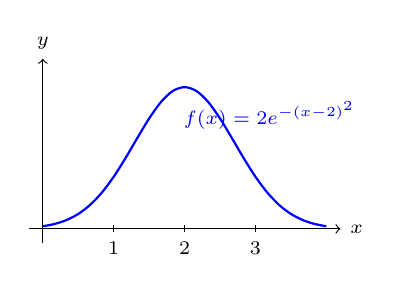
\begin{tikzpicture}[scale=0.9, every node/.style={font=\scriptsize}]
  \draw[->] (-0.2, 0) -- (4.2, 0) node[right] {$x$};
  \draw[->] (0, -0.2) -- (0, 2.4) node[above] {$y$};
  \draw[thick, blue, domain=0:4, smooth] plot (\x, {2*exp(-(\x-2)^2)});
  \foreach \t in {1, 2, 3} \draw (\t, 0.05) -- (\t, -0.05) node[below] {$\t$};
  \node[blue] at (3.2, 1.6) {$f(x) = 2e^{-(x-2)^2}$};
\end{tikzpicture}
\end{center}

\end{document}
